\documentclass{book}

\usepackage[spanish]{babel}
\usepackage[utf8]{inputenc}

\usepackage{graphicx}
\usepackage{lipsum}
\usepackage{microtype}

\usepackage[T1]{fontenc}
\usepackage{lmodern}

\usepackage[pdftex]{hyperref}

\hypersetup{pdfauthor={J. S. Castellanos Durám},pdftitle={RECANEWS Volumen 2 - Febrero 2015},colorlinks,linkcolor=black,urlcolor=blue}

\usepackage[paperwidth=210mm, paperheight=297mm, textwidth=160mm, textheight=240mm, bindingoffset=1cm]{geometry}


% obliczenie szerokości lewego marginesu
\usepackage{calc}
\newlength{\lmargin}
\setlength{\lmargin}{1in + \hoffset + \oddsidemargin}

\usepackage{flowfram}

\usepackage{color}

\usepackage{tikz}
\usepackage{anyfontsize}

% definicja ramek typu flow umieszczonych na stonie 1
\newflowframe[1]{8cm}{31\baselineskip}{-.50cm}{0\baselineskip}[frame1-1a]
\newflowframe[1]{8cm}{23\baselineskip}{8.5cm}{0\baselineskip}[frame1-2b]
%\newflowframe[1]{5cm}{27\baselineskip}{11cm}{0\baselineskip}[frame1-3c]

%definicja ramek statycznych wstawianych na stronie 1
\newstaticframe[1]{\paperwidth}{14cm}{-\lmargin}{12.5cm}[frameS-1a]
\newstaticframe[1]{14cm}{7\baselineskip}{0cm}{45\baselineskip}[frameS-1b]

%definicja ramki dymamicznej wstawiania na stonie nieparzystej
\newdynamicframe[odd]{2cm}{2cm}{-\lmargin}{6cm}[frameD-1a]
%definicja ramki dymamicznej wstawiania na stonie parzystej
\newdynamicframe[even]{2cm}{2cm}{\textwidth+\lmargin-2cm}{6cm}[frameD-1b]

% definicja ramek typu flow na kolejnych stronach
\newflowframe[>1]{8cm}{57\baselineskip}{-.50cm}{0\baselineskip}[frame2-1a]
\newflowframe[>1]{8cm}{57\baselineskip}{8.5cm}{0\baselineskip}[frame2-2a]
%\newflowframe[>1]{5cm}{57\baselineskip}{11cm}{0\baselineskip}[frame2-3a]

\definecolor{green}{rgb}{0.6,0.8,0.1}

\title{RECANEWS Volumen 2 - Febrero 2015}
\author{J. Sebastián Castellanos Durán}
\date{\relax}

\begin{document}

\pagestyle{empty}

% wstawienie numerów stron w ramki dynamiczne frameD-1a i frameD-1b
\begin{dynamiccontents*}{frameD-1a}
\begin{tikzpicture}
\draw(0,0) node [fill=purple, minimum width=2cm, minimum height=2cm]{
{\sffamily\bfseries\Huge\color{white}\thepage}
};
\end{tikzpicture}
\end{dynamiccontents*}

\begin{dynamiccontents*}{frameD-1b}
\begin{tikzpicture}
\draw(0,0) node [fill=purple, minimum width=2cm, minimum height=2cm]{
{\sffamily \bfseries\Huge\color{white}\thepage}
};
\end{tikzpicture}
\end{dynamiccontents*}


% wstawienie grafiki w ramkię statyczną frameS-1a
\begin{staticcontents*}{frameS-1a}
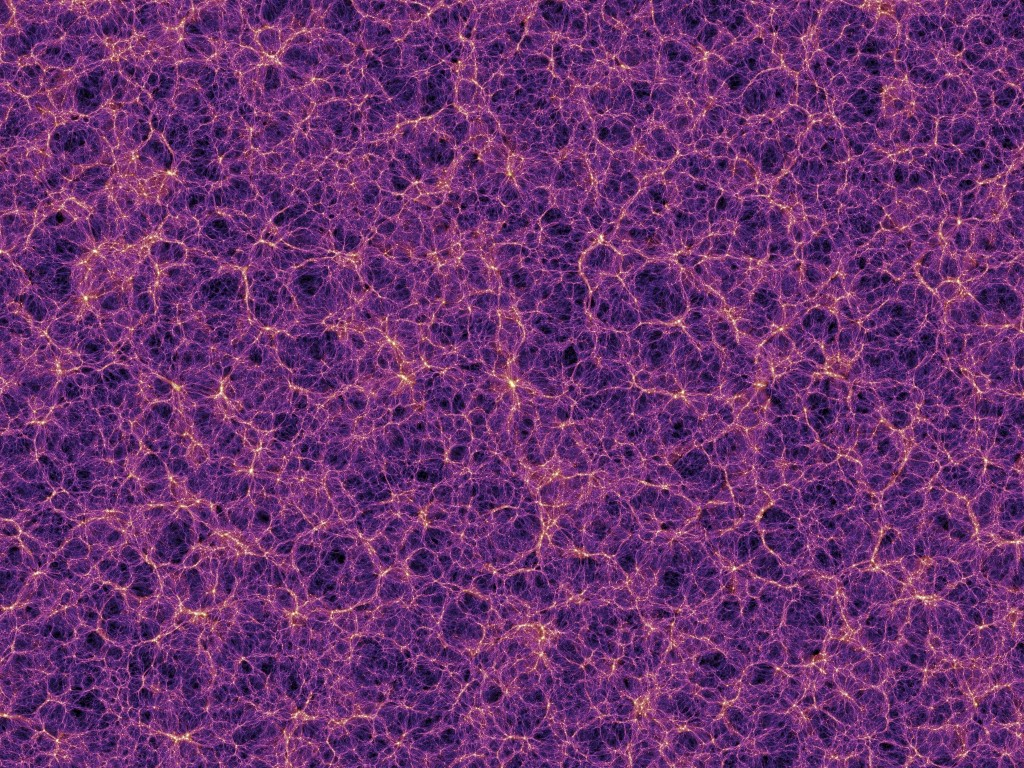
\includegraphics[viewport = {0cm 0cm 21cm 16cm}, clip]{fig1.jpg}
\end{staticcontents*}

% wypełnienie tekstem ramki statycznej frameS-1b
\begin{staticcontents*}{frameS-1b}
\begin{tikzpicture}
\draw(0,0) node [fill=white, text width=13cm, inner sep=5mm, opacity=0.7]{
\large\sffamily
{\fontsize{70}{30}\selectfont {\color{black} RECANEWS}}\\


{\fontsize{30}{30}\selectfont {\color{black} Volumen 2}}\\


\begin{flushright}
{\fontsize{30}{30}\selectfont {\color{black} Febrero 2015}}
\end{flushright}
};
\end{tikzpicture}
\end{staticcontents*}

\tableofcontents{}
% wlanie tekstu do wszystkich ramek typu flow



\newpage


\renewcommand\thesection{\arabic{section}}
\renewcommand\thesubsection{\arabic{subsection}}

%*********************************************
\addcontentsline{toc}{section}{Noticias Astronomía y ciencias del espacio en Colombia}
\section*{Noticias Astronomía y ciencias del espacio en Colombia}
%*********************************************

\subsection{Nueva Postdoc en el grupo de Astronomía. U Andes.}

Veronica Arias es la nueva Postdoc del grupo de Astronomía de la Universidad de los Andes, Trabajara con Jaime Forero en el plano de galaxias satélite de Andrómeda, enfocándose en los posibles orígenes de ese tipo de estructuras. Veronica estudió Física en la Universidad Nacional realizó su trabajo de grado en simulaciones de galaxias satélite, con Rigoberto Casas Miranda. Posteriormente realizó el Doctorado en hamburgo, en el Hamburger Sternwarte, de la Universidad de Hamburgo, en simulaciones hidrodinámicas de atmósferas de objetos sub estelares, Realizó un Postdoctorado en el Sydney institute for Astronomy, de la Universidad de Sydney, allí trabajó con Geraint Lewis en el plano de galaxias satélite que orbitan la galaxia de Andrómeda enfocándose en la estabilidad de ese tipo de estructuras.\\

\begin{flushright}
Grupo de Astronomía Universidad de los Andes, Bogota
\end{flushright}

\subsection{Programación del Seminario de\\ Astronomía en el planetario\\ (Spacio).}

Ya esta lista la programaciones del Seminario de Astronomía en el planetario (Spacio) a realizarse todos los sábados a las 4 pm en las instalaciones del planetario de Bogotá a partir del Sabado 7 de Febrero.\\

\noindent La programación completa puede ser descargada por medio de los siguientes links:

\begin{itemize}
\item \url{http://goo.gl/i0aSCw}
\item \url{http://goo.gl/kQmbHc}
\end{itemize}


\begin{flushright}
Nicolas Garavito
\end{flushright}

\subsection{Escuela Andina de Cosmología\\ Junio 1 - 26, 2015, Bogotá\\ Universidad de los Andes\\ Deadline 28 Febrero}

Me complace enviarles este correo para invitarlos a participar en la Escuela Andina de Cosmología que se realizará del 1 al 26 de Junio 2015 en Bogotá, Colombia.\\

\noindent Esperamos reunir estudiantes de la región con expertos en el área de cosmología tanto observacional como numérica y teórica.
El objetivo no es solamente enseñar tópicos avanzados en estos temas sino también explorar la posibilidad de enfrentarse a problemas reales de investigación en colaboración con los expositores invitados.\\

\noindent La escuela está dirigida a estudiantes que ya tengan conocimientos básicos de cosmología y de programación. Tenemos en mente un nivel de pregrado-licenciatura avanzado, maestría o doctorado.\\

\noindent En la siguiente página van a encontrar la lista de instructores invitados, los temas que esperamos cubrir y el enlace al formulario de pre-inscripción con fecha límite el 28 de febrero.\\

\noindent \url{http://forero.github.io/AndeanCosmologySchool/}\\

\noindent Por favor compartan este correo con personas que puedan estar interesadas.\\

\begin{flushright}
Jaime Forero
\end{flushright}

\subsection{1st workshop on Current Challenges in Cosmology: Inflation and the Origin of CMB anomalies.\\ Mayo 18 - 22, 2015 Cali, Colombia}

\textbf{Main topics}
\begin{itemize}
\item Statistical anisotropy and anisotropic expansion
\item Primordial magnetic fields
\item Parity violation and polarization in the CMB
\item Effective field theory of inflation
\item Anisotropic non-gaussianity
\item CMB data analysis
\item Primordial Gravitational  Waves
\item Galileons and Horndeski theories
\end{itemize}

Contacto:\\
\begin{flushright}
\url{juanpbeltran@uan.edu.co}\\
\url{cesar.valenzuela@correounivalle.edu.co}\\
\url{yeinzon.rodriguez@uan.edu.co}
\end{flushright}
\newpage
\subsection{XVIII Festival de Astronomía\\20-22 de Febrero 2015\\Villa de Leyva - Boyacá}

El Festival de astronomía en Villa de Leyva convoca a miles de aficionados y profesionales de las ciencias del espacio que año tras año se reúnen en este Patrimonio Histórico y Cultural de la Nación para compartir e intercambiar conocimientos y experiencias con todas las personas que se interesa por los temas espaciales.\\

\noindent El cielo oculto en el brillo de las luces de las grandes ciudades esconde un maravilloso cielo estrellado. Pero no hay que perder la ilusión de ver miles de estrellas en una noche, pues puede encontrarse en sitios alejados de luz artificial. Como es costumbre, cada año en busca de cielos oscuros la Asociación de Astrónomos Autodidactas - ASASAC emprende su viaje a Villa de Leyva, que ofrece una cálida plaza y la oportunidad de apagar las luces para disfrutar de un cielo nocturno. La zona más brillante es la Vía Láctea, objeto del cielo que inspiró múltiples historias mitológicas y del cuál hace parte nuestro Sistema Solar.\\

\noindent En esta edición el Festival de Astronomía tiene como tema central la celebración de los 50 años de nuestra Asociación que nos ha llevado a través de la divulgación de esta ciencia a conocer, compartir y fascinar tanto a entendidos como neófitos con las maravillas del cosmos. Además, nos unimos a la UNESCO en la celebración del Año Internacional de la Luz.

\noindent Más Información:
\begin{center}
\url{http://goo.gl/cMVOQs}
\end{center}


\subsection{Nuevo repositorio Github para RECANEWS}

Ya Se encuentra listo el repositorio en Github del RECANEWS el cual se podrá consultar la versión pdf de cualquiera de los Volúmenes de RECANEWS.\\

Repositorio: \url{https://github.com/recanews}\\



%*********************************************
\newpage

\addcontentsline{toc}{section}{Programas de posgrados}
\section*{Programas de posgrados}
%*********************************************


\subsection{Inscripciones Abiertas Maestria en Astronomía en el Observatorio\\ Astronómico Nacional y en Fisica\\ Universidad Nacional de Colombia}

\begin{itemize}
\item Pago de derechos de inscripción \\
\textbf{HASTA EL 13 DE ABRIL DE 2015}
\item Formalización de la inscripción\\
\textbf{DESDE EL 9 DE FEBRERO}\\
\textbf{HASTA EL 13 DE ABRIL DE 2015}
\end{itemize}

Mas Informacion:
\begin{center}
\url{http://admisiones.unal.edu.co/}
\end{center}


\begin{flushright}
J. Sebastian Castellanos Duran
\end{flushright}

%*********************************************
\addcontentsline{toc}{section}{Congresos y eventos}
\section*{Congresos y eventos}
%*********************************************

\subsection{EWASS 2015\\ Deadline: 10 March 2015}

The European Week of Astronomy and Space Science (EWASS, formerly JENAM) is the annual meeting of the European Astronomical Society (EAS). With more than 20 years of tradition, it has imposed itself as the largest conference for European astronomy. In addition to plenary sessions and the award of prestigious prizes, the conference hosts many symposia held in parallel, as well as special sessions and meetings.\\

\noindent The EAS together with one of its affiliated societies, organises the annual EWASS conference to enhance its links with national communities, to broaden connections between individual members and to promote European networks.\\

\noindent EWASS 2015 is held for the first time in Tenerife, Spain and is expected to welcome over 600 astrophysicists from all over Europe and even beyond.\\

\noindent Más información:
\begin{center}
\url{ http://eas.unige.ch/EWASS2015/index.jsp}
\end{center}

%*********************************************
\newpage
\addcontentsline{toc}{section}{Escuelas}
                   \section*{Escuelas}
%*********************************************

\subsection{ASTRON/JIVE Summer Student Programme 2015\\ Deadline February 9, 2015.}

The Netherlands Institute for Radio Astronomy (ASTRON) and the Joint Institute for VLBI in Europe (JIVE) announce the availability of a limited number of grants for their 2015 Summer Research Programme. The Programme enables astronomy students (graduate or advanced undergraduate) to spend the summer (10-12 weeks) at the Dwingeloo Observatory, conducting astronomical research under the supervision of ASTRON and JIVE staff members. Possible topics of study include radio galaxies and quasars, aspects of observational cosmology, continuum and line emission/absorption from normal and starburst galaxies, faint radio sources, pulsars, molecular clouds, cosmic magnetism, as well as working with LOFAR data. The actual project the successful candidate will work on will be defined after arrangement with the local supervisor. The programme is not aimed at engineering or electronics students.
\noindent Más información: \begin{center}
\url{http://www.astron.nl/astronomy-group/astronjive-summer-student-programme}
\end{center}

%*********************************************

\addcontentsline{toc}{section}{¿Cómo publicar en RECANEWS?}
\section*{¿Cómo publicar en RECANEWS?}
%*********************************************

Para publicar en RECANEWS se debe enviar un correo a reca.news@gmail.com con las siguientes especificaciones:
\begin{description}
\item[Correo:]reca.news@gmail.com
\item[Asunto:]Título de la publicación
\item[Contenido:]Contenido de la publicación\\
Persona encargada (Opcional)\\
Correo de la persona encargada (Opcional)
\end{description}
  
\noindent Más información sobre RECANEWS

\begin{center}
\url{http://goo.gl/Fb8UEc}
\end{center}


%*********************************************
\addcontentsline{toc}{section}{Contacto del RECA}
\section*{Contacto del RECA:}
%*********************************************

\begin{description}
\item[Correo RECA:]\url{reca.astronomia@gmail.com}
\item[Facebook:] \url{https://www.facebook.com/RECAstronomia}
\item[Google$+$:] \url{http://goo.gl/P0DEf4}
\item[Twitter:] \url{https://twitter.com/RECAstronomia}
\item[Pagina Web:] \url{http://goo.gl/Fl4zQP}
\end{description}


%*********************************************
\addcontentsline{toc}{section}{Representantes de RECA en las regiones}
\section*{Representantes de RECA en las regiones}
%*********************************************
\begin{description}
\item[Medellín:]Malory Agudelo Vásquez\\
\url{magudelov@gmail.com}\\ \url{magudelov@fisica.udea.edu.co}
\item[Pereira:]Luisa Fernanda Cardona\\ \url{luisferncardona@utp.edu.co}
\item[Pasto:]Katherine Mafla Oliva\\
\url{skmofis13@gmail.com}
\item[Cali:]Daniel Santacruz
\item[Bogotá:]Maria Camila Remolina Gutierrez\\
\url{mc.remolina197@uniandes.edu.co}\\

Andres Felipe Ramos Padilla\\
\url{andresrp25@gmail.com}\\

Juan David Jimenez Nieto\\
\url{jdjimenezn@correo.udistrital.edu.co}
\end{description}


%*********************************************
\addcontentsline{toc}{section}{Editor RECANEWS}
			\section*{Editor RECANEWS}
%********************************************
  
\begin{flushright}
J. Sebastián Castellanos Durán\\
\url{jsebastian405@gmail.com}
\end{flushright}
\begin{flushright}
Cualquier comentario por favor escribir al correo  \url{reca.news@gmail.com}\\
Febrero 2015
\end{flushright}


\end{document}


